\documentclass{beamer}

\mode<presentation> {

%\usetheme{default}
%\usetheme{AnnArbor}
%\usetheme{Antibes}
%\usetheme{Bergen}
%\usetheme{Berkeley}
%\usetheme{Berlin}
%\usetheme{Boadilla}
\usetheme{CambridgeUS}
%\usetheme{Copenhagen}
%\usetheme{Darmstadt}
%\usetheme{Dresden}
%\usetheme{Frankfurt}
%\usetheme{Goettingen}
%\usetheme{Hannover}
%\usetheme{Ilmenau}
%\usetheme{JuanLesPins}
%\usetheme{Luebeck}
%\usetheme{Madrid}
%\usetheme{Malmoe}
%\usetheme{Marburg}
%\usetheme{Montpellier}
%\usetheme{PaloAlto}
%\usetheme{Pittsburgh}
%\usetheme{Rochester}
%\usetheme{Singapore}
%\usetheme{Szeged}
%\usetheme{Warsaw}

%\usecolortheme{albatross}
\usecolortheme{beaver}
%\usecolortheme{beetle}
%\usecolortheme{crane}
%\usecolortheme{dolphin}
%\usecolortheme{dove}
%\usecolortheme{fly}
%\usecolortheme{lily}
%\usecolortheme{orchid}
%\usecolortheme{rose}
%\usecolortheme{seagull}
%\usecolortheme{seahorse}
%\usecolortheme{whale}
%\usecolortheme{wolverine}

%\setbeamertemplate{footline} % To remove the footer line in all slides uncomment this line
%\setbeamertemplate{footline}[page number] % To replace the footer line in all slides with a simple slide count uncomment this line
\setbeamertemplate{navigation symbols}{} % To remove the navigation symbols from the bottom of all slides uncomment this line
}

\usepackage{graphicx}
\usepackage{multimedia}
\usepackage{booktabs}
\usepackage{float}
\usepackage{tikz}
\usepackage{scalefnt}
\usepackage{listings}
\usepackage{todonotes}
\usepackage{tabularx}
\usepackage{enumitem}
\usepackage{hyperref}
\usepackage{xcolor}
\usepackage{caption}

\makeatletter
\renewcommand\verbatim@font{\color{red}\normalfont\ttfamily}
\makeatletter


\setitemize{label=\usebeamerfont*{itemize item}
\usebeamercolor[fg]{itemize item}
\usebeamertemplate{itemize item}}

\definecolor{ao(english)}{rgb}{0.0, 0.5, 0.0}
\definecolor{aureolin}{rgb}{0.99, 0.93, 0.0}
\definecolor{bostonuniversityred}{rgb}{0.8, 0.0, 0.0}

\renewcommand{\tabularxcolumn}[1]{>{\small}m{#1}}
\renewcommand{\arraystretch}{2}

%% Listings definition for Go language
%% Go language reference : http://www.golang.org
%% Author : Uriel Corfa <uriel@corfa.fr>
%% Project home: https://bitbucket.org/korfuri/golang-latex-listings

\lstdefinelanguage{go}{
  % Keywords as defined in the BNF
  morekeywords=[1]{break,default,func,interface,%
    case,defer,go,map,struct,chan,else,goto,package,%
    switch,const,fallthrough,if,range,type,continue,%
    for,import,return,var,select},
  % Special identifiers, builtin functions
  morekeywords=[2]{make,new,nil,len,cap,copy,complex,%
    real,imag,panic,recover,print,println,iota,close,%
    closed,_,true,false,append,delete},
  % Basic types
  morekeywords=[3]{%
    string,int,uint,uintptr,double,float,byte,%
    int8,int16,int32,int64,int128,%
    uint8,uint16,uint32,uint64,uint128,%
    float32,float64,complex64,complex128,%
    rune},
  % Strings : "toto", 'toto', `toto`
  morestring=[b]{"},
  morestring=[b]{'},
  morestring=[b]{`},
  % Comments : /* comment */ and // comment
  comment=[l]{//},
  morecomment=[s]{/*}{*/},
  % Options
  sensitive=true
}

\lstset{
  language={go},
  basicstyle=\ttfamily\tiny
}

\title[Fuzzing with afl]{\textbf{Modern Fuzzing with \texttt{afl}}}

\author{}
\institute[]
{
Anish Kunduru \\
Jon Osborne \\
Nik Kinkel \\
\medskip
}
\date{\today}

\begin{document}

\begin{frame}
\titlepage
\end{frame}

% Slide 1
\begin{frame}
\frametitle{Introduction to Fuzzing}
\begin{columns}
\column{.4\textwidth}
\begin{itemize}
\item{Purpose and methods of fuzzing}
\item{Detecting unique state transitions}
\begin{itemize}
\item{fault detection}
\item{error detection}
\end{itemize}
\item{Application-specific data formats}
\begin{itemize}
\item{efficiency of tests}
\end{itemize}
\end{itemize}
\column{.6\textwidth}
\begin{figure}
\centering{
	\scalefont{0.85}
	\scalebox{0.55}{% Graphic for TeX using PGF
% Title: /home/linuxlite/Documents/ComS417/417paper/slides/figures/RIPR.tex
% Creator: Dia v0.97.2
% CreationDate: Mon Apr 18 00:03:29 2016
% For: linuxlite
% \usepackage{tikz}
% The following commands are not supported in PSTricks at present
% We define them conditionally, so when they are implemented,
% this pgf file will use them.
\ifx\du\undefined
  \newlength{\du}
\fi
\setlength{\du}{15\unitlength}
\begin{tikzpicture}
\pgftransformxscale{1.000000}
\pgftransformyscale{-1.000000}
\definecolor{dialinecolor}{rgb}{0.000000, 0.000000, 0.000000}
\pgfsetstrokecolor{dialinecolor}
\definecolor{dialinecolor}{rgb}{1.000000, 1.000000, 1.000000}
\pgfsetfillcolor{dialinecolor}
\pgfsetlinewidth{0.100000\du}
\pgfsetdash{}{0pt}
\pgfsetdash{}{0pt}
\pgfsetbuttcap
\pgfsetmiterjoin
\pgfsetlinewidth{0.100000\du}
\pgfsetbuttcap
\pgfsetmiterjoin
\pgfsetdash{}{0pt}
\definecolor{dialinecolor}{rgb}{1.000000, 1.000000, 1.000000}
\pgfsetfillcolor{dialinecolor}
\fill (-44.017742\du,1.249427\du)--(-44.017742\du,3.249427\du)--(-42.082258\du,3.249427\du)--(-42.082258\du,1.249427\du)--cycle;
\definecolor{dialinecolor}{rgb}{0.000000, 0.000000, 0.000000}
\pgfsetstrokecolor{dialinecolor}
\draw (-44.017742\du,1.249427\du)--(-44.017742\du,3.249427\du)--(-42.082258\du,3.249427\du)--(-42.082258\du,1.249427\du)--cycle;
\pgfsetbuttcap
\pgfsetmiterjoin
\pgfsetdash{}{0pt}
\definecolor{dialinecolor}{rgb}{0.000000, 0.000000, 0.000000}
\pgfsetstrokecolor{dialinecolor}
\draw (-44.017742\du,1.249427\du)--(-44.017742\du,3.249427\du)--(-42.082258\du,3.249427\du)--(-42.082258\du,1.249427\du)--cycle;
% setfont left to latex
\definecolor{dialinecolor}{rgb}{0.000000, 0.000000, 0.000000}
\pgfsetstrokecolor{dialinecolor}
\node[anchor=west] at (-44.000000\du,0.849427\du){Fuzzer};
\pgfsetlinewidth{0.100000\du}
\pgfsetdash{}{0pt}
\pgfsetdash{}{0pt}
\pgfsetbuttcap
{
\definecolor{dialinecolor}{rgb}{0.000000, 0.000000, 0.000000}
\pgfsetfillcolor{dialinecolor}
% was here!!!
\pgfsetarrowsend{to}
\definecolor{dialinecolor}{rgb}{0.000000, 0.000000, 0.000000}
\pgfsetstrokecolor{dialinecolor}
\draw (-42.082258\du,2.249427\du)--(-39.200000\du,2.249427\du);
}
% setfont left to latex
\definecolor{dialinecolor}{rgb}{0.000000, 0.000000, 0.000000}
\pgfsetstrokecolor{dialinecolor}
\node[anchor=west] at (-38.200000\du,1.399427\du){};
% setfont left to latex
\definecolor{dialinecolor}{rgb}{0.000000, 0.000000, 0.000000}
\pgfsetstrokecolor{dialinecolor}
\node[anchor=west] at (-37.150000\du,2.449427\du){};
% setfont left to latex
\definecolor{dialinecolor}{rgb}{0.000000, 0.000000, 0.000000}
\pgfsetstrokecolor{dialinecolor}
\node[anchor=west] at (-39.950000\du,11.299427\du){};
% setfont left to latex
\definecolor{dialinecolor}{rgb}{0.000000, 0.000000, 0.000000}
\pgfsetstrokecolor{dialinecolor}
\node[anchor=west] at (-38.700000\du,2.349427\du){Test Case};
% setfont left to latex
\definecolor{dialinecolor}{rgb}{0.000000, 0.000000, 0.000000}
\pgfsetstrokecolor{dialinecolor}
\node[anchor=west] at (-32.700000\du,0.349427\du){};
% setfont left to latex
\definecolor{dialinecolor}{rgb}{0.000000, 0.000000, 0.000000}
\pgfsetstrokecolor{dialinecolor}
\node[anchor=west] at (-41.500000\du,8.500000\du){Binary};
% setfont left to latex
\definecolor{dialinecolor}{rgb}{0.000000, 0.000000, 0.000000}
\pgfsetstrokecolor{dialinecolor}
\node[anchor=west] at (-37.214271\du,10.099427\du){};
% setfont left to latex
\definecolor{dialinecolor}{rgb}{0.000000, 0.000000, 0.000000}
\pgfsetstrokecolor{dialinecolor}
\node[anchor=west] at (-38.360571\du,8.923479\du){Reachability?};
% setfont left to latex
\definecolor{dialinecolor}{rgb}{0.000000, 0.000000, 0.000000}
\pgfsetstrokecolor{dialinecolor}
\node[anchor=west] at (-37.750000\du,11.750000\du){Infection?};
% setfont left to latex
\definecolor{dialinecolor}{rgb}{0.000000, 0.000000, 0.000000}
\pgfsetstrokecolor{dialinecolor}
\node[anchor=west] at (-38.250000\du,14.600000\du){Propagation?};
\pgfsetlinewidth{0.100000\du}
\pgfsetdash{}{0pt}
\pgfsetdash{}{0pt}
\pgfsetbuttcap
{
\definecolor{dialinecolor}{rgb}{0.000000, 0.000000, 0.000000}
\pgfsetfillcolor{dialinecolor}
% was here!!!
\pgfsetarrowsend{to}
\definecolor{dialinecolor}{rgb}{0.000000, 0.000000, 0.000000}
\pgfsetstrokecolor{dialinecolor}
\draw (-36.250000\du,12.150000\du)--(-36.265902\du,13.685000\du);
}
% setfont left to latex
\definecolor{dialinecolor}{rgb}{0.000000, 0.000000, 0.000000}
\pgfsetstrokecolor{dialinecolor}
\node[anchor=west] at (-38.250000\du,17.150000\du){Revealability?};
\pgfsetlinewidth{0.100000\du}
\pgfsetdash{}{0pt}
\pgfsetdash{}{0pt}
\pgfsetbuttcap
{
\definecolor{dialinecolor}{rgb}{0.000000, 0.000000, 0.000000}
\pgfsetfillcolor{dialinecolor}
% was here!!!
\pgfsetarrowsend{to}
\definecolor{dialinecolor}{rgb}{0.000000, 0.000000, 0.000000}
\pgfsetstrokecolor{dialinecolor}
\draw (-36.250000\du,15.150000\du)--(-36.265902\du,16.685000\du);
}
\pgfsetlinewidth{0.100000\du}
\pgfsetdash{}{0pt}
\pgfsetdash{}{0pt}
\pgfsetmiterjoin
\definecolor{dialinecolor}{rgb}{0.000000, 0.000000, 0.000000}
\pgfsetstrokecolor{dialinecolor}
\draw (-38.686671\du,8.100000\du)--(-38.686671\du,17.726982\du)--(-33.586671\du,17.726982\du)--(-33.586671\du,8.100000\du)--cycle;
\pgfsetlinewidth{0.100000\du}
\pgfsetdash{}{0pt}
\pgfsetdash{}{0pt}
\pgfsetbuttcap
{
\definecolor{dialinecolor}{rgb}{0.000000, 0.000000, 0.000000}
\pgfsetfillcolor{dialinecolor}
% was here!!!
\pgfsetarrowsend{to}
\definecolor{dialinecolor}{rgb}{0.000000, 0.000000, 0.000000}
\pgfsetstrokecolor{dialinecolor}
\draw (-36.250000\du,9.350000\du)--(-36.265902\du,10.885000\du);
}
\pgfsetlinewidth{0.100000\du}
\pgfsetdash{}{0pt}
\pgfsetdash{}{0pt}
\pgfsetmiterjoin
\pgfsetbuttcap
{
\definecolor{dialinecolor}{rgb}{0.000000, 0.000000, 0.000000}
\pgfsetfillcolor{dialinecolor}
% was here!!!
\pgfsetarrowsend{to}
\definecolor{dialinecolor}{rgb}{0.000000, 0.000000, 0.000000}
\pgfsetstrokecolor{dialinecolor}
\pgfpathmoveto{\pgfpoint{-35.486671\du}{2.276982\du}}
\pgfpathcurveto{\pgfpoint{-30.886671\du}{2.226982\du}}{\pgfpoint{-36.036671\du}{2.376982\du}}{\pgfpoint{-36.336671\du}{7.926982\du}}
\pgfusepath{stroke}
}
% setfont left to latex
\definecolor{dialinecolor}{rgb}{0.000000, 0.000000, 0.000000}
\pgfsetstrokecolor{dialinecolor}
\node[anchor=west] at (-47.686671\du,18.226982\du){No fault? or illegal state?};
\pgfsetlinewidth{0.100000\du}
\pgfsetdash{}{0pt}
\pgfsetdash{}{0pt}
\pgfsetmiterjoin
\pgfsetbuttcap
{
\definecolor{dialinecolor}{rgb}{0.000000, 0.000000, 0.000000}
\pgfsetfillcolor{dialinecolor}
% was here!!!
\pgfsetarrowsend{to}
\definecolor{dialinecolor}{rgb}{0.000000, 0.000000, 0.000000}
\pgfsetstrokecolor{dialinecolor}
\pgfpathmoveto{\pgfpoint{-36.386671\du}{18.014482\du}}
\pgfpathcurveto{\pgfpoint{-36.336671\du}{19.314482\du}}{\pgfpoint{-42.136671\du}{20.414482\du}}{\pgfpoint{-43.236671\du}{18.614482\du}}
\pgfusepath{stroke}
}
\end{tikzpicture}
}
}
\end{figure}
\end{columns}
\end{frame}

% Slide 2
\begin{frame}
\frametitle{TODO}

% TODO

\end{frame}

% Slide 3
\begin{frame}[fragile]
\frametitle{american fuzzy lop (\texttt{afl})}

\begin{columns}[c]

\column{0.5\textwidth}

\textbf{Goal}: find unique crashes.

\begin{itemize}
    \item Efficiency is coverage.
    \item Syntax is hard.
    \item State transitions matter.
    \item Automatic feedback loop is critical.
\end{itemize}

\column{0.5\textwidth}

\begin{center}
\begin{figure}
\begin{verbatim}
        _____.__   
_____ _/ ____\  |  
\__  \\   __\|  |  
 / __ \|  |  |  |__
(____  /__|  |____/
     \/            
\end{verbatim}
\end{figure}
\end{center}

\end{columns}

\end{frame}

% Slide 4
\begin{frame}
\frametitle{TODO}

% TODO

\end{frame}

% Slide 5
\begin{frame}
\frametitle{Core Operation}

\begin{columns}[c]

\column{0.5\textwidth}

\begin{itemize}
    \item Pruned test case input queue
    \item Spawn new cow processes
    \item Save unique crashes and hangs
\end{frame}

\end{columns}

% Slide 6
\begin{frame}
\frametitle{Fuzzing Strategies}
\begin{itemize}

\item{Deterministic}
	\begin{itemize}
	\item{Bit and byte flips, arithmetic operations, and known integers}
	\item{Easy to reach states used for more advanced techniques}
	\end{itemize}

\item{Random}
	\begin{itemize}
	\item{Randomized operations performed in a sequential loop}
	\item{More time consuming}
	\item{Greater propagation in program states}
	\item{Consists of stacked tweaks and splicing}
	\end{itemize}

\end{itemize}

\end{frame}

% Slide 7
\begin{frame}
\frametitle{\texttt{afl} in Action}

\begin{columns}

\column{0.4\textwidth}

\begin{itemize}
\item{Increased security}
\begin{itemize}
\item{Mozilla Firefox}
\item{OpenSSH}
\end{itemize}
\item{Can also be used to test program stability}
\end{itemize}

\column{0.6\textwidth}

\begin{center}
\begin{table}
\caption{\texttt{afl} Trophy Case}
\tiny
\begin{tabular}{c | c | c}
Firefox & Internet Explorer & Safari \\
OpenSSH & Putty & OpenSSL \\
GnuPG & bash & Adobe Flash \\
sqlite & PHP & libpng \\
nginx & JavascriptCore & ffmpeg \\
iOS / ImageIO & Android / libstagefright & VLC \\
redis & perl & wireshark \\
Linux ext4 & glibc & llvm \\
\end{tabular}
\caption*{...and many more}
\end{table}
\end{center}

\end{columns}
\end{frame}

% Slide 8
\begin{frame}[fragile]
\frametitle{Practical Evaluation}

\begin{columns}[c]

\column{0.4\textwidth}

\begin{figure}
\vspace*{-0.5cm}
\caption{Message structure}
\vspace*{-0.85cm}
\begin{lstlisting}[language=C,frame=single]
typedef struct {
    (*@\texttt{\color{blue}uint8\_t}@*)  type;
    (*@\texttt{\color{blue}uint8\_t}@*)  addr_len;
    (*@\texttt{\color{blue}uint8\_t}@*)  uname_len;
    (*@\texttt{\color{blue}uint16\_t}@*) len;
    (*@\texttt{\color{blue}char}@*)    *addr;
    (*@\texttt{\color{blue}char}@*)    *uname;
} msg_t;
\end{lstlisting}
\end{figure}

\begin{figure}
\vspace*{-1cm}
\caption{Vulnerable parsing code}
\vspace*{-1cm}
\begin{lstlisting}[language=C,frame=single]
// UNSAFE read
memcpy(msg->addr,
       &(buf[idx]),
       msg->addr_len);
idx += msg->addr_len;
msg->addr[msg->addr_len] = '\0';
// UNSAFE read
memcpy(msg->uname,
       &(buf[idx]),
       msg->uname_len);
msg->uname[msg->uname_len] = '\0';
// UNSAFE write
memset(buf, 0, msg->len);
\end{lstlisting}
\end{figure}


\column{0.6\textwidth}

\begin{center}
\begin{figure}
\vspace*{-0.6cm}
\caption{\texttt{afl} run}
\vspace*{-0.5cm}
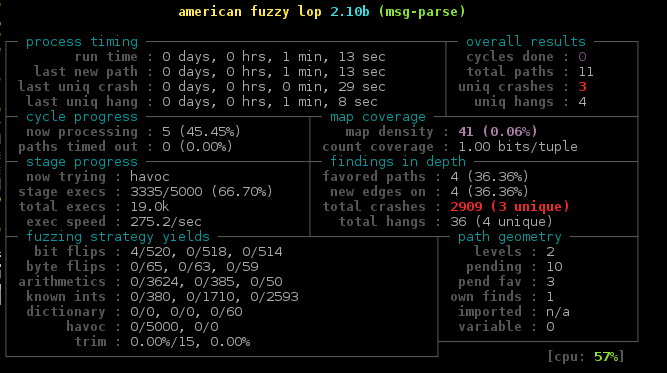
\includegraphics[scale=0.32]{../figures/afl-run}
\end{figure}
\end{center}

\begin{center}
\begin{varwidth}{0.7\textwidth}
\begin{figure}
\vspace*{-1cm}
\begin{lstlisting}[numbers=none]
01 (*@\SoulColor\hl{9c}@*) 02 00 23 6e 57 47 59 50 51 49
53 63 57 47 6c 49 35 71 6b 42 59 4b
4b 36 31 76 58 56 68 73 6f 57 68\end{lstlisting}
\caption{\texttt{afl}-generated Test Case}
\end{figure}
\end{varwidth}
\end{center}


\end{columns}


\end{frame}

% Slide 9
\begin{frame}
\Huge{\centerline{Questions}}
\end{frame}


\end{document} 
